\section{Works Done}
\label{sec:worksDone}
This week is most related to proposal report writing, chart drawing and project plan construction. In addition these works, some of us also make progress in some practical applications.
\subsection{Mechanics}
This week some other mechanical designs were introduced. One of them is using the gear for the door. The simple drawing for the design can be seen from Fig \ref{}

\begin{figure}
    \centering
    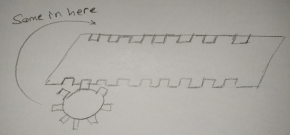
\includegraphics{img/mechDoga1.png}
    \caption{Door Design}
    \label{fig:mechDoga1}
\end{figure}

By using at least two gears we can move the door back and forth. However, there exist a problem of some of the foods can block the door while it is closing. This problem can be fixed by making a thin slit around the door. By this way, the door cannot fall or lost its connection with the gear. Moreover, since the slits are narrow, cat food cannot get into the slits and block the door. Although it blocks the door somehow, the system will come equilibrium since other cat foods also jam between the door and the slit which will stop the food flow eventually. 
The main problem of this design is the mass of the foods since when the door is closed the considerable amount of food will be on the door and it will create a force on the door. Therefore the door will get into contact with the lower part of the slit and this will create friction between the door and the slit. One has to apply high torque in order to move the door. The problem starts here. Our motor might not be enough to create that torque. Although there exist some motor that can deal with that force we don’t prefer it since it will have high power consumption and its price will be high compared with low power motors.
This week also we have also attempted to try the design of our old design, which was the salt cup idea. Cardboard was cut according to the design specifications but still, the tests aren't done. It is planned to be done next week. According to the result of the test, other designs might gain importance.


\subsection{Proposal Report}
To write proposal report, we create a work division among team. The aim was to distribute the work such that everyone will try to expert in his/her own area and make the best. Therefore, we developed work packages and shared based on the skills.

More information on work distribution and personal responsibilities are given in section \ref{sec:workDistribution}. The works are given in figure \ref{fig:ganttChart} as Gantt charts.

\begin{figure}
    \centering
    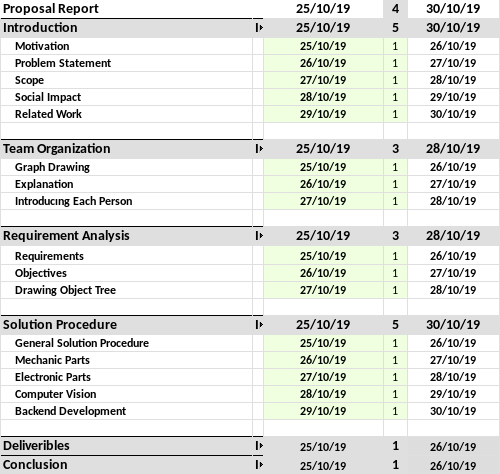
\includegraphics[width=\linewidth]{img/proposalGanttChart.png}
    \caption{Proposal Gantt Chart}
    \label{fig:ganttChart}
\end{figure}

We realized that solution procedure part may be misunderstood which is why we contacted with our supervisor. However at the moment the report is being written, we do not know the correct way to improve it, therefore it is left to the next week to edit this part.